\section{Tofu na kuskusie z sezonową sałatką}
\bigskip
\small
\begin{minipage}{0.45\textwidth}
    \noindent \textbf{Czas:} 30 minut \\
    \textbf{Poziom trudności:} umiarkowany
\end{minipage}
\begin{minipage}{0.45\textwidth}
    \noindent \textbf{Ilość sprzątania:} średnia\\
    \textbf{Wymagany mysi sprzęt:} -
\end{minipage}
\normalsize
\vspace{0.5cm}

\begin{multicols}{2}

\subsection*{Składniki}
\begin{itemize}
    \item 1 porcja kaszy kuskus
    \item 1 kostka tofu (naturalnego, wędzonego, lub w gotowej marynacie)
    \item mix sałat
    \item garść pomidorków koktajlowych lub 1 duży, dojrzały pomidor
    \item 1 ogórek gruntowy
    \item 0.5 czerwonej cebuli
    \item zielona cebulka wedle uznania
    \item 1 duży ząbek czosnku przeciśnięty przez praskę
    \item 1 łyżka miodu
    \item przyprawy
    \item olej do smażenia
    \item odrobina oliwy i soku z cytryny
    \item 0.5 kostki bulionu warzywnego lub drobiowego
    \item sól i pieprz do smaku
\end{itemize}

\columnbreak

\begin{figure}[H]
    \centering
    \fbox{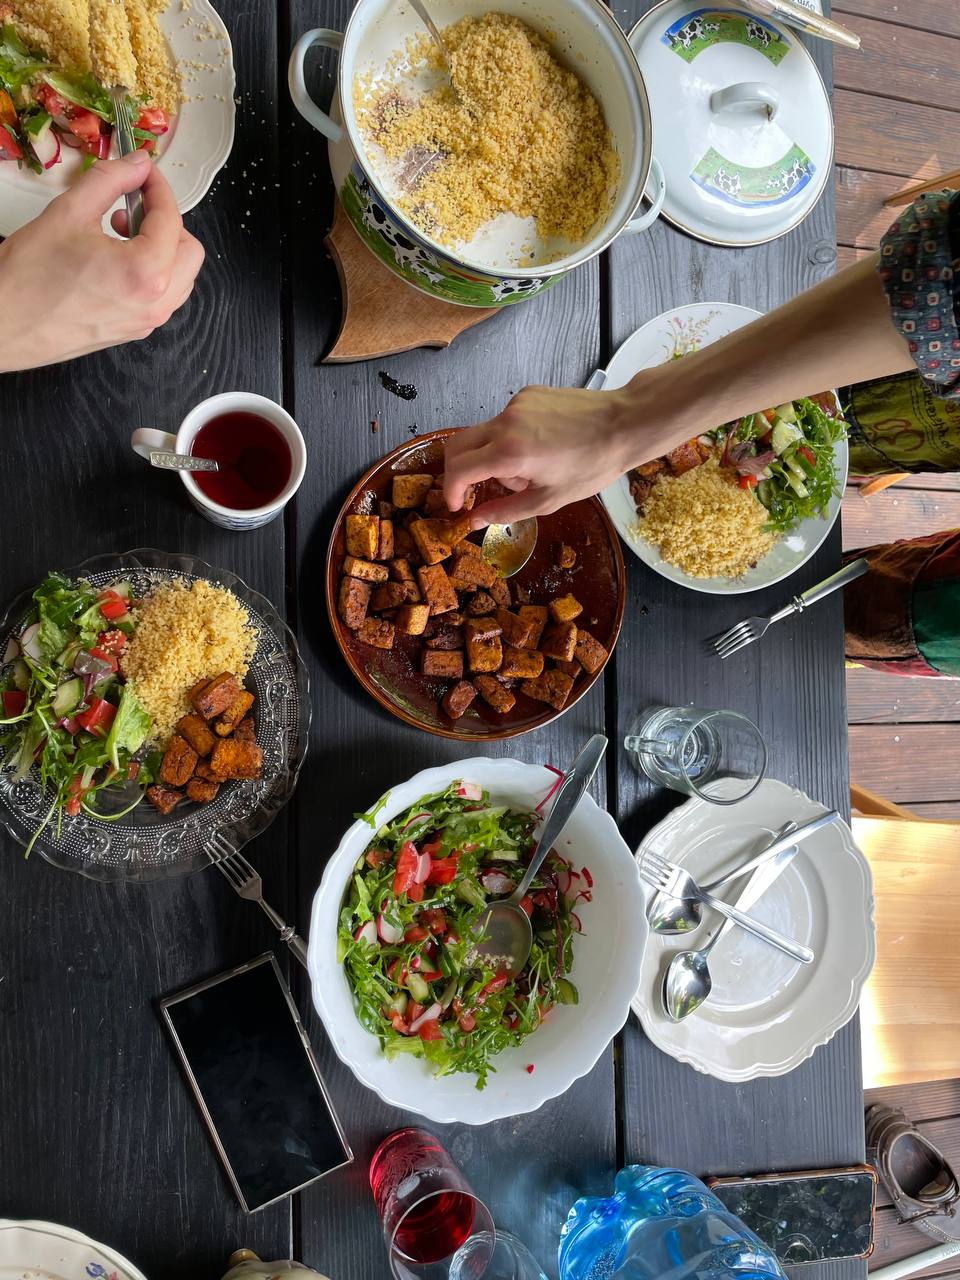
\includegraphics[width=0.45\textwidth]{images/tofu.jpg}}
\end{figure}
\end{multicols}

\vspace{0.5cm}

\subsection*{Instruktaż}
\begin{enumerate}
    \item Sałatkę i tofu przygotować osobno zgodnie z przepisem znajdującym się na ostatniej pozycji w spisie treści.
    \item W kubku odmierzyć odpowiednią porcję kaszy kuskus na 1 osobę i podsmażać wraz z połową łyżeczki pieprzu na niewielkiej ilości oliwy i małym ogniu do momentu zarumienienia się kaszy, lub przez ok. 3 minuty. Następnie zdjąć z ognia i zalać taką samą objętościowo ilością wody, uprzednio rozpuszczając w niej bulion i szczyptę soli. Całość przykryć i pozostawić na ok. 5 minut.
    \item W razie potrzeby kaszę dosolić do smaku i podawać z tofu oraz sałatką
\end{enumerate}

\vspace{0.5cm}

\small
\subsection*{Propozycja podania}
Z posiekaną zieloną cebulką, z natką pietruszki, z domowym sosem czosnkowym.

\vspace{0.3cm}

\subsection*{Dodatkowe uwagi}
Nie mam uwag.

\newpage
